\documentclass{sigchi}

% Use this command to override the default ACM copyright statement
% (e.g. for preprints).  Consult the conference website for the
% camera-ready copyright statement.


%% EXAMPLE BEGIN -- HOW TO OVERRIDE THE DEFAULT COPYRIGHT STRIP -- (July 22, 2013 - Paul Baumann)
% \toappear{Permission to make digital or hard copies of all or part of this work for personal or classroom use is      granted without fee provided that copies are not made or distributed for profit or commercial advantage and that copies bear this notice and the full citation on the first page. Copyrights for components of this work owned by others than ACM must be honored. Abstracting with credit is permitted. To copy otherwise, or republish, to post on servers or to redistribute to lists, requires prior specific permission and/or a fee. Request permissions from permissions@acm.org. \\
% {\emph{CHI'14}}, April 26--May 1, 2014, Toronto, Canada. \\
% Copyright \copyright~2014 ACM ISBN/14/04...\$15.00. \\
% DOI string from ACM form confirmation}
%% EXAMPLE END -- HOW TO OVERRIDE THE DEFAULT COPYRIGHT STRIP -- (July 22, 2013 - Paul Baumann)


% Arabic page numbers for submission.  Remove this line to eliminate
% page numbers for the camera ready copy 

\pagenumbering{arabic}

% Load basic packages
\usepackage{balance}  % to better equalize the last page
\usepackage{graphics} % for EPS, load graphicx instead 
%\usepackage[T1]{fontenc}
\usepackage{txfonts}
\usepackage{times}    % comment if you want LaTeX's default font
\usepackage[pdftex]{hyperref}
% \usepackage{url}      % llt: nicely formatted URLs
\usepackage{color}
\usepackage{textcomp}
\usepackage{booktabs}
\usepackage{ccicons}
\usepackage{todonotes}
\usepackage{soul}
\usepackage{paralist}
\usepackage{listings}

\usepackage{caption}
\usepackage{subcaption}
\usepackage[super]{nth}
\usepackage{amsmath}

% llt: Define a global style for URLs, rather that the default one
\makeatletter
\def\url@leostyle{%
  \@ifundefined{selectfont}{\def\UrlFont{\sf}}{\def\UrlFont{\small\bf\ttfamily}}}
\makeatother
\urlstyle{leo}

% To make various LaTeX processors do the right thing with page size.
\def\pprw{8.5in}
\def\pprh{11in}
\special{papersize=\pprw,\pprh}
\setlength{\paperwidth}{\pprw}
\setlength{\paperheight}{\pprh}
\setlength{\pdfpagewidth}{\pprw}
\setlength{\pdfpageheight}{\pprh}

% Make sure hyperref comes last of your loaded packages, to give it a
% fighting chance of not being over-written, since its job is to
% redefine many LaTeX commands.
\definecolor{linkColor}{RGB}{6,125,233}
\hypersetup{%
  pdftitle={SIGCHI Conference Proceedings Format},
  pdfauthor={LaTeX},
  pdfkeywords={SIGCHI, proceedings, archival format},
  bookmarksnumbered,
  pdfstartview={FitH},
  colorlinks,
  citecolor=black,
  filecolor=black,
  linkcolor=black,
  urlcolor=linkColor,
  breaklinks=true,
}

% create a shortcut to typeset table headings
% \newcommand\tabhead[1]{\small\textbf{#1}}

% End of preamble. Here it comes the document.
\begin{document}

\title{Measuring Interaction Design\\
Measuring Interaction before developing prototypes\\
Measuring Interaction Graphs}

\numberofauthors{2}
\author{%
  \alignauthor{1st Author Name\\
    \affaddr{Affiliation}\\
    \affaddr{City, Country}\\
    \email{e-mail address}}\\
  \alignauthor{2nd Author Name\\
    \affaddr{Affiliation}\\
    \affaddr{City, Country}\\
    \email{e-mail address}}\\
}

\maketitle

\begin{abstract}
  Early development of prototypes of user interfaces is good
  practice. However, they have to cover specific usage scenarios, and
  because they are limited in focus, the whole picture of the user
  interface is easily lost. Even simple questions dealing with number
  and length of interaction paths or impact of possible user errors
  can be answered only for the specific scenarios being analysed.

  We present a tool that transforms models of a user interface into a
  graph. This is then used to specify usage scenarios, and to generate
  possible interaction paths. Metrics based on possible paths, with or
  without possible mistakes, can be easily computed. When applying
  these metrics get precise and objective values that can be used to
  compare designs or to identify weakness. When applying them to mail
  applications, we learn for example that Gmail has \hl{7 times more
  optimal paths, it has 4x more paths include at most one possible
  user error, that it has 20\% fewer steps.}

  
\end{abstract}

\keywords{Experimental; Evaluation; Statecharts: UML; UML-IDEA; Testing.}

\category{H.5.1}{Information interfaces and presentation (e.g., HCI)}{Multimedia Information Systems}. 
\category{H.5.2}{Information interfaces and presentation (e.g.,
  HCI)}{User Interfaces}. 

\section{Introduction}

\begin{quote}
  Subcommittee: Technology, Systems, and Engineering

People we should pay particular attention to:
Caroline Appert
Conversy, St�phane
Nebeling, Michael

Keyword we need to pay attention to:
This subcommittee will focus on technology, systems and engineering
contributions that enable, improve, or advance interaction. This will
include software and hardware technologies and systems that enable and
demonstrate novel interactive capabilities, as well as languages,
methods and tools for \hl{CONSTRUCTION AND ENGINEERING} of interactive
systems. Engineering contributions should clearly demonstrate how they
address interactive systems concerns such as, for example,
scalability, reliability, interoperability, testing, and
performance. Systems and technology contributions will be judged by
their technical innovation and/or ability to connect, SIMPLIFY or
enrich interactions, for example in intelligent interfaces and
mobile/ubiquitous computing.

\end{quote}


We present an approach that allows a designer to assess interaction
design (IxD) qualities such as efficiency, consistency,
error-proneness and recovery from premature committment. Key
importance is given to the ability to quickly
\begin{inparaenum}[(a)]
\item understand how supportive a user interface (UI) is with respect
  to user efficiency;
\item understand how prone the UI is to user navigation
  errors;
\item understand how recoverable the UI is from those errors; and,
\item support task analysis and task/scenario design.
\end{inparaenum}
%
This allows different designs to be objectively compared to support
designers in the construction and engineering of interactive
systems. To explain our work we present a comparison of four different
web mail front ends. We have chosen this domain because it is very
well known and yet several trivial questions lead to non trivial
results. We applied the same techniques also in other domains, such as
HVAC and other embedded UIs.

The approach is based on UML statechart models of UIs which are
automatically processed to produce \emph{interaction graphs}. These
are then used to specify interaction scenarios and unfold interaction
paths (called \emph{execution traces}) determined by the specific
scenarios being considered. Traces are fed to several graph-theoretic
computations which produce a dashboard with different results with the
answers. Except for development of models and specification of the
desired scenarios, which have to be done manually, the other steps are
totally automatic; models of a design (such as the ones shown in the
paper) could be developed in a matter of a couple of hours.

Developing good UIs for web or mobile applications is a
complex and expensive endeavour. One reason is the combination of
devices, interaction modalities and workflows that need to be
supported.
%
Adopting Usage Centred Development practices is effective, as is
following established design principles~\cite{constantine99}. In
particular, one of the most effective technique is early
prototyping~\cite{buxton07} to explore part of the five-dimensional
prototyping space~\cite{mccurdy06}. It is particularly effective when
paired with usability investigations based on user testing or
heuristic evaluations~\cite{rubin08,preece02}.

However, it requires prototypes which are usually developed with
certain tasks in mind, and therefore are quite restricted in terms of
depth, breadth, dynamics and data. Furthermore, in addition to the
possible bias introduced by prototypes, usability results are always
surrounded by a cloud of uncertainty, due to subjectivity introduced
by participants and facilitators or by other contingency factors
involved in the analysis. Thus, although a  significant effort
needs to be expended to develop and use prototypes, less than optimal
results are obtained. 

Even worse, there might be questions whose answer cannot be easily
found. For example, given one or more potential IxD solutions and some
usage scenarios, interesting questions could include: ``How many
different ways can be followed by the user to carry out the scenario?'', ``Which
are the shortest ones?'', ``If a user makes a mistake, would he or she
be able to recover?'', ``How many steps would the recovery
require?''. When designing and evaluating embedded UIs (such as when
dealing with plane's cockpits~\cite{conversy07}), other relevant
questions might include ``How would the above properties change if we
add a certain a widget?'', or ``... if we replace a widget with
another?''.  At the moment, even these straightforward questions are
quite complicated to answer. In fact, they require development of
prototypes, inspecting them, manual tracking of which screens and
widgets are used at which stage, and a systematic manual analysis.

This should not be the case, however. These answers provide important
insights to a designer, and potentially support assements of potential user
flexibility, user efficiency, error proneness, ability to recover,
compactness and consistency of a design.

Our contribution consists of the development of a tool that transforms
models and scenario specifications into interaction paths, and the
definition of metrics that provide concise, precise and objective
measures of a design. The examples included in the paper show that
among four web mail applications, and with respect to a typical usage
scenario, Gmail is the most efficient and flexible UI, with the best
ability to recover from certain mistakes. In fact, Gmail has the
largest number of shortest sequences of steps (even when users are
supposed to make 1 or 2 mistakes), but when users make more than 2
mistakes the number of paths drops significantly; on average, best and worst
cases, Gmail features also shorter paths, requiring \hl{CHECK 20\% fewer steps};
however, the probability that a user hits an optimal path with Gmail
is almost half of that of another application, and the probability
that a random walker hits a state that is not due to a mistake is
\hl{SAY SOMETHING}.
%
These values suggest that Gmail offers more ways to accomplish tasks
included in the scenario, that comparably more of these ways do not
involve extra steps, that they require fewer steps, and that it might
be more difficult for novice users to exploit the most efficient
ways. Further inspections show that some differences are due to the
slightly different interaction structures adopted for uploading
messages. If Gmail didn't exist yet, its designers could obtain these
answers well before performing usability studies.

\section{Background}
\label{sec:background}

(right now these are random notes)

SwingState: work done by 
Caroline Appert\cite{appert2008swingstates}

in java, FSA used as a conceptual framework to write the code of
widgets so that events and event handlers in the ui can more easily be
conceived, developed and verified.

They say: StateCharts were used in the StateMaster User Interface
Management System [40], and a variant of them specifically tailored to
designing user interfaces was used in the more recent HsmTk toolkit
[18]. StateCharts however are significantly more complicated and hard
to learn than plain state machines, and our experience is that user
interface designers and developers have difficulties exploiting their
power. Other approaches include Petri Nets [41], which have also been
used to specify user interfaces, for example in the PetShop system
[42]. Here too, the learning curve is steep, making the adoption of
such a model by developers difficult.

With SwingStates, any number of state machines can run simulateneously. A state machine
can be active, i.e., handling the events it receives, or inactive,
i.e., ignoring events

We adopt a similar apporach, but using UML state machine (which are
more powerful than FSA) for conceiving, guiding development, analysis
and verification of the behavior of the entire app.

Nebeling says:\cite{nebeling2011metrics}

Despite the fact that screen sizes and average screen resolutions have
dramatically increased over the past few years, little attention has
been paid to the design of web sites for large, high-resolution
displays that are now becoming increasingly used both in enterprise
and consumer spaces. We present a study of how the visual area of the
browser window is currently utilised by news web sites at different
widescreen resolutions. The analysis includes measurements of space
taken up by the article content, embedded ads and the remaining
components as they appear in the viewport of the web browser. The
results show that the spatial distribution of page elements does not
scale well with larger viewing sizes, which leads to an increasing
amount of unused screen real estate and unnecessary scrolling. We
derive a number of device-sensitive metrics to measure the quality of
web page layout in different viewing contexts, which can guide the
design of flexible layout templates that scale effectively on large
screens.

Stephane Conversy\cite{conversy07} says: (friend of nicolas roussel in
the committee)

ARINC 661 provides precise information for communication protocol
between application (called User Applications) and user interface
components (called widgets) as well as precise information about the
widgets themselves. However, in ARINC 661, no information is given
about the behaviour of these widgets and about the behaviour of an
application made up of a set of such widgets.

The purpose of ARINC 661 specification (ARINC 661, 2002) is to define
interfaces to a Cockpit Display System (CDS) used in interactive
cockpits that are now under

application of a formal description technique to the various elements
of ARINC 661 specification within an industrial project. This formal
description technique called Interactive Cooperative Objects defines
in a precise and non-ambiguous way all the elements of ARINC 661
specification. The application of the formal description techniques is
shown on an interactive application called MPIA (Multi Purpose
Interactive Application). Within this application, we present how ICO
are used for describing interactive widgets, User Applications and
User Interface servers (in charge of interaction techniques). The
emphasis is put on the model-based management of the feel of the
applications allowing rapid prototyping of the external presentation
and the interaction techniques.

The Interactive Cooperative Objects (ICOs) formalism is a formal
description technique dedicated to the specification of interactive
systems [4, 11]. It uses concepts borrowed from the object-oriented
approach to describe the structural or static aspects of systems, and
uses high-level Petri nets [8] to describe their dynamic or
behavioural aspects.

The Interactive Cooperative Objects (ICOs) formalism is a formal
description technique dedicated to the specification of interactive
systems [4, 11]. It uses concepts borrowed from the object-oriented
approach to describe the structural or static aspects of systems, and
uses high-level Petri nets [8] to describe their dynamic or
behavioural aspects.

Voida\cite{voida} says:
We describe an alternative model for organizing the
desktop interface-activity-based computing-and
identify a series of high-level system requirements for
interfaces that use activity as their primary organizing
principle.

We could mention this work when we introduce scenarios, and say that
people inventing these new metaphors could take advantage of our
metrics if they model 2+ apps. 

Eg. they say: Requirement 2. Activity-based systems should provide
lightweight mechanisms to create, change, and alter
activities, since heavyweight interaction techniques are
likely to deter adoption and use.

eg Requirement 7. Because information sharing is a
�common case� in knowledge work, lightweight sharing
capabilities should be integrated directly as a first-class
interaction technique. 

\section{Generation of interaction paths}
\label{sec:traces}

\begin{quote}
  here we describe how we transform state machines into graphs, how we
  specify scenarios, how the system computes traces, how metrics are
  computed. 
\end{quote}

Notice that a scenario specifies only the desired occurrences of user
actions, not the necessary ones. For example, the model specifies that
in order to view a conversation while reading another one, one has to
\texttt{goBack} to the inbox first. It is the task of MIGTOOL to
unfold cyles in the graph and compute all the  paths that connect the
desired user actions. 

Actions specified in a scenario are called \texttt{bridges}, because
they represent one or more edges in the graph that have to be followed
when carrying out the 


\section{Comparing applications}
\label{sec:casestudy}

In this section we describe some examples based on well known web mail
clients, namely Gmail, Horde, SquirrelMail and Roundcube. We chose
these examples because they are very well known, and therefore are
easy to describe and understand. And yet, despite email being a very
well understood domain, the kind of questions that can be posed and
the answers that are found provide an insight on some of the usability
properties of these applications. 

\subsection{Models and scenarios}
\label{sec:models-scenarios}

Models of the four applications have been manually developed using UML
state machines. In order to support a fair comparison, all four models
cover the same set of use cases: listing the content of the inbox,
reading a message or conversation, replying to a message, composing
and sending a new message.

Figure~\ref{fig:model} shows part of the model of Gmail. At some
point, the user might be viewing all the conversations of the inbox
(state \texttt{viewingConversations}); available actions include
moving to the next or previuous block of conversations, refreshing the
list, or opening a specific conversation (transition
\texttt{open(conversation)}). This transition (which is assumed to
occur when the user clicks on one of the visible conversations) leads
to the state \texttt{viewingAConversation}, where the behavior of the
system is defined by a more detailed state machine. By default the
user is viewing a conversation, but by performing the \texttt{reply}
action the UI moves to a state called \texttt{replying}, where the
body of the message can be typed, the subject can be changed, or
another addressee can be added.

Notice that this behavior ``happens'' in one of the two concurrent
regions specified by this model. In parallel to this, the user can
either be reading messages (state \texttt{reading}) or may be
composing a new message (state \texttt{composing}). In the latter case
the user can independently add recipients, attachments, write the body
or subject of the message; and send or cancel it.

\begin{figure*}[tbh]
  \centering
  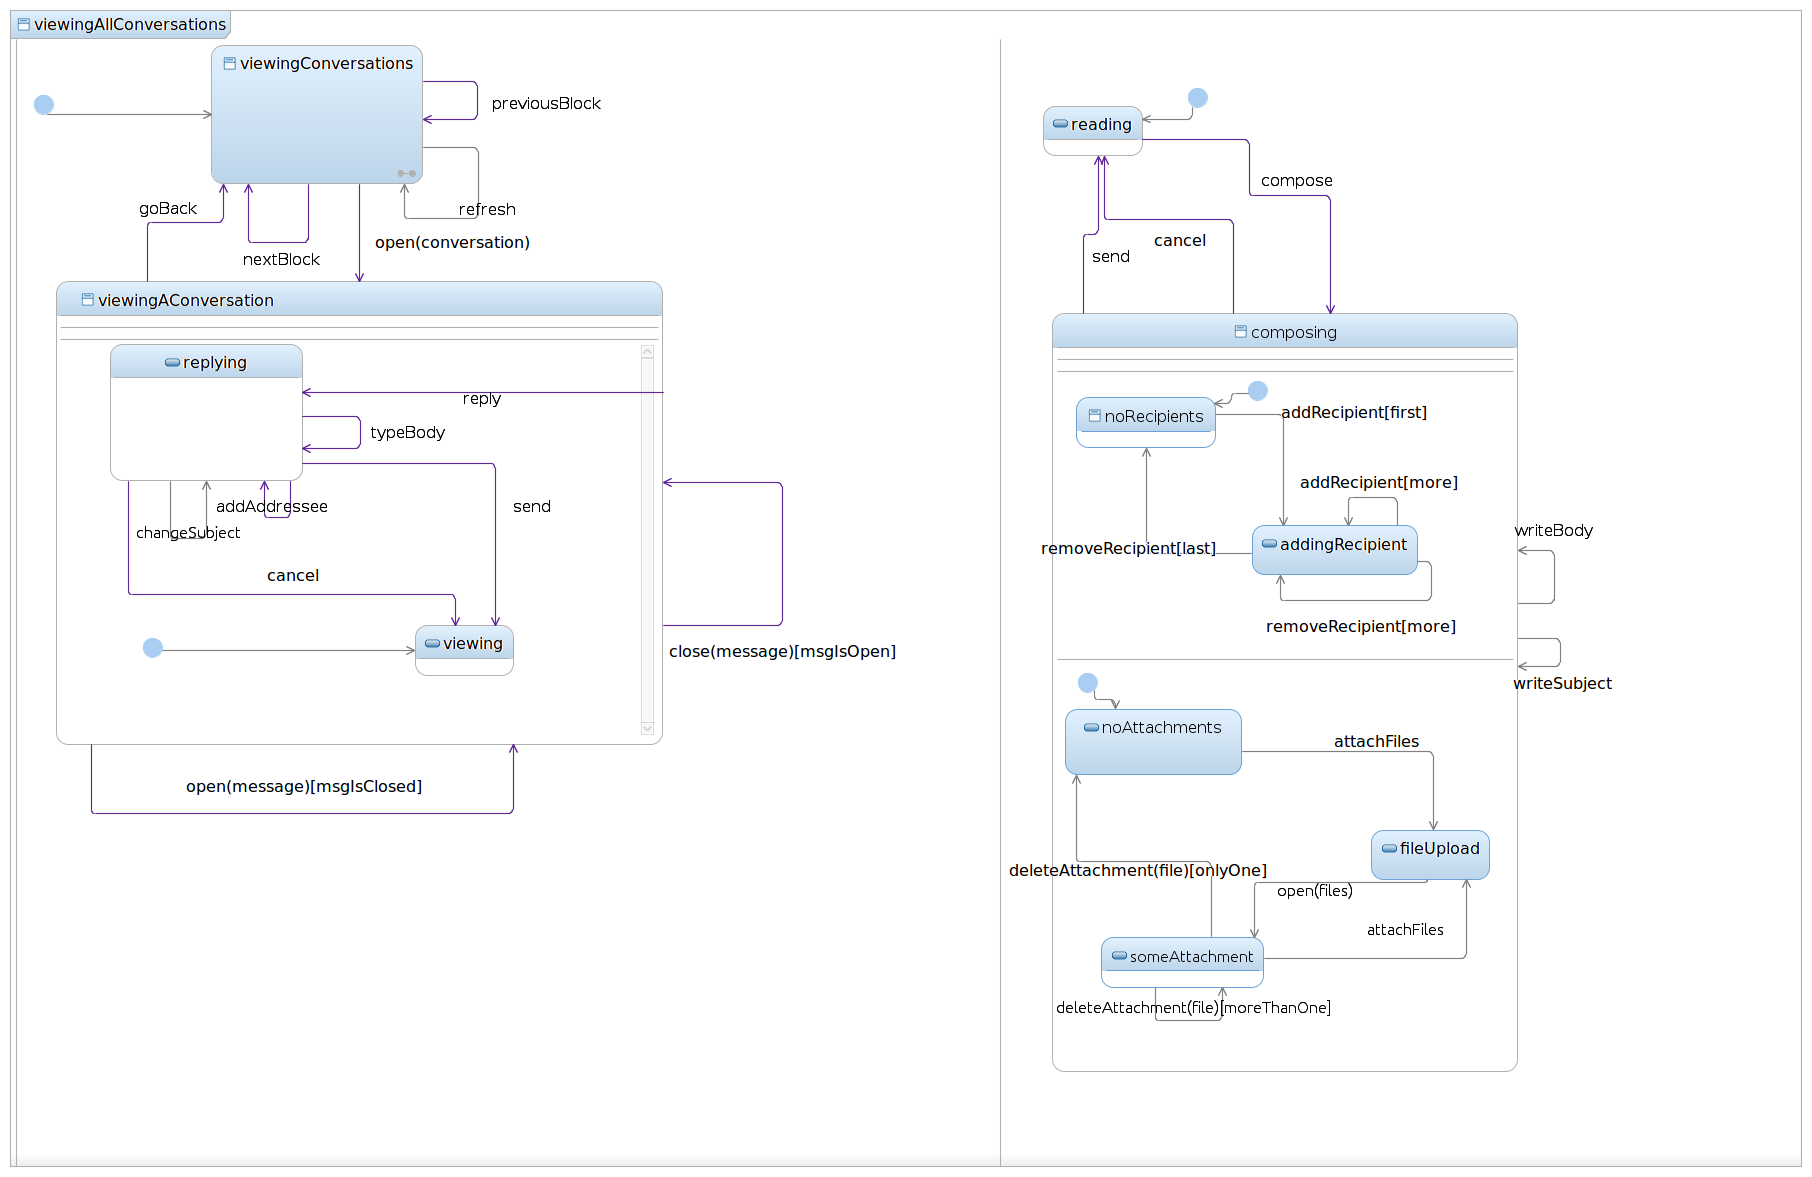
\includegraphics[width=\linewidth]{figures/gmail_2.png}
  \caption{Part of the Gmail model.}\label{fig:model}
\end{figure*}

The model that we show here is part of what we used in the examples
reported below, and that is only a part of what the real Gmail
application supports. The actual model that we used consists of 
24 states, 12 pseudo states, 12 regions, and 61 transitions. 

The flattening process, which takes a fraction of a second on a
low-cost PC, produces a directed multigraph with 47 vertices and 634
edges; when simplified by collapsing multiple edges between any pair of
vertices, the graph includes 312 edges. Each vertex represents one of
the possible combinations of simple states in any of the regions that
can be active at the same time.

Similar models and corresponding graphs were produced for the other
three applications. 



\subsection{Analysis of interaction designs}
\label{sec:analysis}

Inspection of the interaction graph is not particularly useful because
even for small graphs like the one  obtained from our Gmail model
no particular structure is evident. Figure~\ref{fig:gom} shows a plot
using a circular layout of the 47 states: because of the large
number of cycles that exist among states, edges form an intricated web
of possible action sequences. This in practice greatly reduces usefulness of
typical network analysis metrics, such as \emph{betweenness,
  eccentricity, page-rank, eigenvalue} centrality measures. 

\begin{figure}
  \centering
  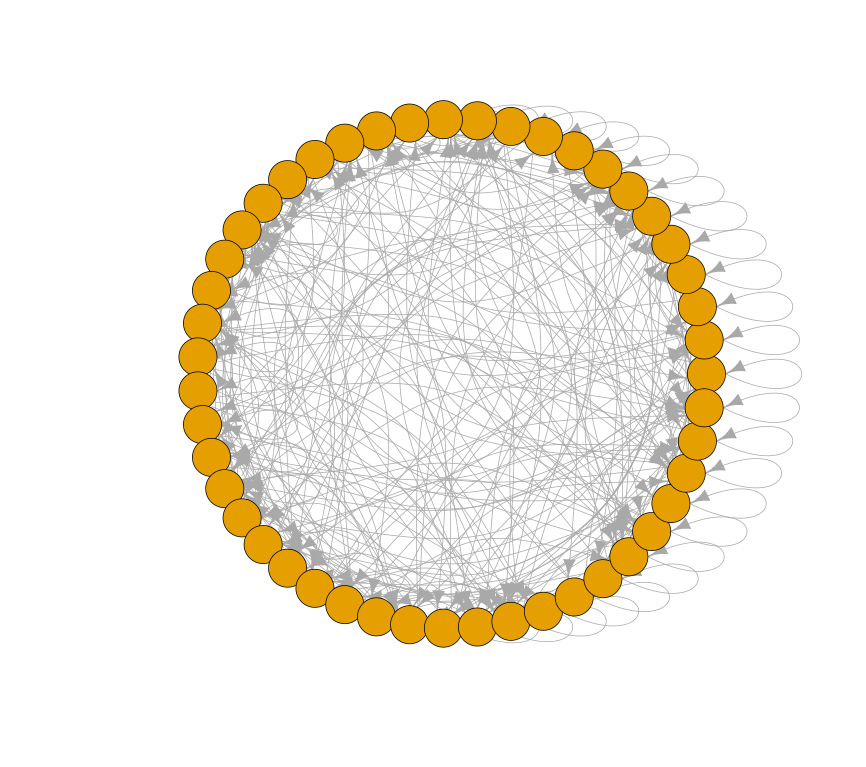
\includegraphics[width=\linewidth]{figures/gom.png}
  \caption{Graph obtained from the Gmail model.}
  \label{fig:gom}
\end{figure}


To be able to obtain results that bear upon usability, we process
further the graph, first by specifying an interaction scenario using
vertices and edges of the graph, and secondly by computing possible
execution paths.

Specification of a scenario consists of formulating it using the
language provided by the graph, i.e. deciding which is the initial
state and which user actions need to be considered. For example, the
following fragment of R code specifies that the scenario should
include, in the given order, two occurrences of
\texttt{open(conversation)}, followed by \texttt{reply}, followed by
\texttt{typeBody}, etc.: \lstset{language=R}
\begin{lstlisting}
edgesWithLabel(gmail,"open(conversation)"),
edgesWithLabel(gmail,"open(conversation)"), 
edgesWithLabel(gmail,"reply"),
edgesWithLabel(gmail,"typeBody"),
edgesWithLabel(gmail,"send"),
edgesWithLabel(gmail,"compose"),
edgesWithLabel(gmail,"addRecipient"),
edgesWithLabel(gmail,"open(files)"),
edgesWithLabel(gmail,"writeBody"),
edgesWithLabel(gmail,"writeSubject"),
edgesWithLabel(gmail,"send")
\end{lstlisting}
In plain language such a scenario means opening one and then a second conversation,
replying to the last message of the second one by typing the body of
the response, sending it, and then composing a new message by adding a
recipient, an attachment, typing the body and subject, and finally
sending it.

The execution traces for such a Gmail scenario, with a detour limit of
3, consist of a graph with 474 vertices and 1753 edges. These traces
entail 12 possible geodesic paths with order 0, 82 with order 1, 30
with order 2 and 33 with order 3. Figure~\ref{fig:numpaths} shows the
number of paths obtained for the four applications, split by detour
order.


\begin{figure}[tbh]
  \centering
  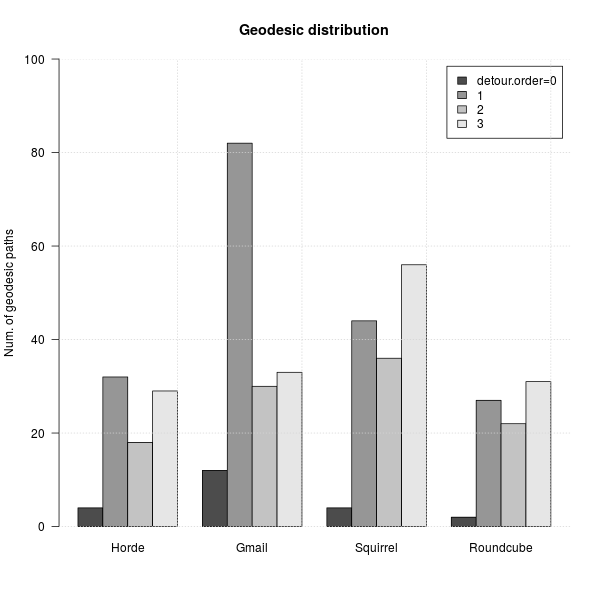
\includegraphics[width=\linewidth]{figures/gpd.png}
  \caption{Number of geodesic paths split by detour order.}
  \label{fig:numpaths}
\end{figure}

% tot.hom
% ##     N min max        M       rel  N
% ## d0  4  15  18 15.75000 0.2539683  4
% ## d1 32  16  22 17.94531 1.7831955 36
% ## d2 18  18  24 19.25000 0.9350649 54
% ## d3 29  19  24 19.95690 1.4531317 83
%  tot.gom
% ##     N min max        M       rel   N
% ## d0 12  13  17 15.08333 0.7955801  12
% ## d1 82  14  24 19.11179 4.2905456  94
% ## d2 30  16  25 20.57778 1.4578834 124
% ## d3 33  17  26 21.51515 1.5338028 157
%  tot.sqm
% ##     N min max        M       rel   N
% ## d0  4  15  19 17.00000 0.2352941   4
% ## d1 44  16  24 19.77273 2.2252874  48
% ## d2 36  18  26 20.88889 1.7234043  84
% ## d3 56  19  25 21.64286 2.5874587 140
%  tot.rcm
% ##     N min max        M       rel  N
% ## d0  2  15  18 16.50000 0.1212121  2
% ## d1 27  16  24 19.07407 1.4155340 29
% ## d2 22  18  25 20.18182 1.0900901 51
% ## d3 31  19  24 21.04839 1.4727969 82

Gmail has the highest number of order 0 and 1 paths, and the highest
difference between the number of order 0 and 1, and between order 1
and 2 (at least 3 times as many order 0 paths than any of the other
applications, and at least twice as many order 1 paths as the any of
the other ones).  Gmail offers 3 times as many error-free alternative
paths to accomplish the scenario, which indicates that users might
more easily follow one of those paths. However, Gmail offers also
almost twice as many order 1 paths, which means that users could be
more easily induced into an erroneous path than when using another
system. Because the number of order 2 or 3 paths decreases, Gmail
reduces therefore the ``error proneness'' of this UI, for executions
that involve 2 or 3 errors. Notice that Roundcube has the smallest
number of order 0 paths (2 of them), which means that users are not
given much flexibility and freedom in carrying out correctly the
scenario.
For none of the systems a detour leads to dead-ends preventing the
user to complete the scenario.

Figure~\ref{fig:bestcase} shows the length of paths in the best case,
i.e., when users would always choose the shortest route. Gmail offers
the shortest paths across the four detour orders (for order 0 the
length is 13 steps; for order 3 the length is 17 steps; the other
applications are remarkably similar among them).  A plausible
interpretation is therefore that Gmail not only offers many more
error-free paths, but also gives the shortest ones. Users are given
more flexibility and more efficiency.

\begin{figure}[htb]
  \centering
  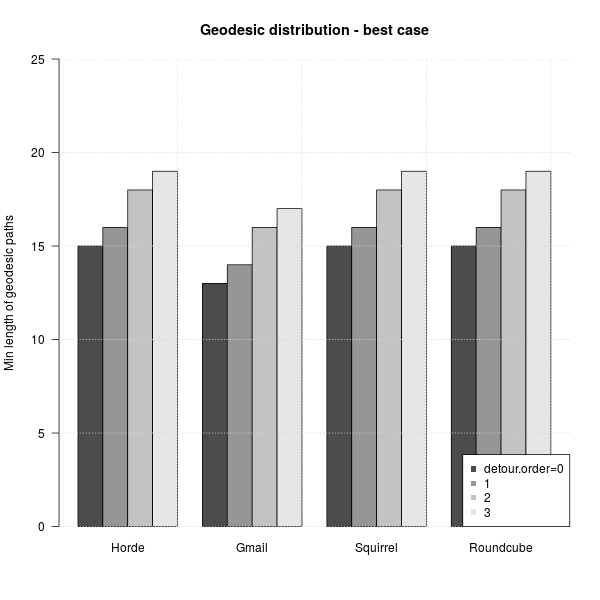
\includegraphics[width=\linewidth]{figures/min-paths.png}
  \caption{Minimum length of  geodesic paths split by detour order.}
  \label{fig:bestcase}
\end{figure}

%Figure~\ref{fig:averagecase} 


% \begin{figure}[htb]
%   \centering
%   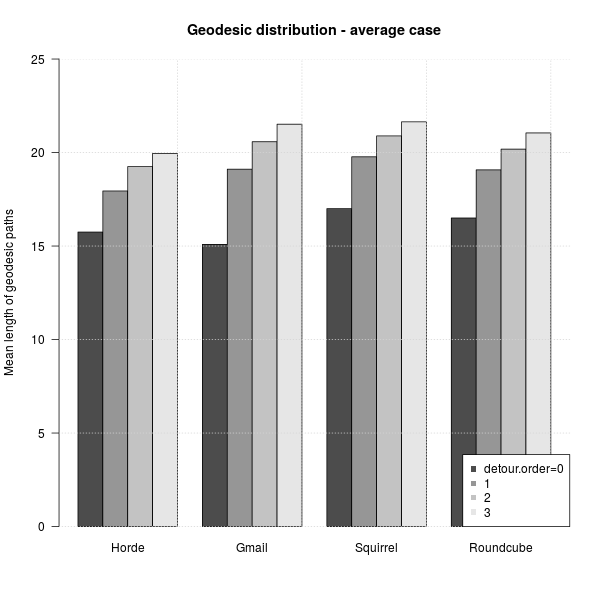
\includegraphics[width=\linewidth]{figures/mean-paths.png}
%   \caption{Average length of  geodesic paths split by detour order.}
%   \label{fig:averagecase}
% \end{figure}

\begin{figure}
  \centering
  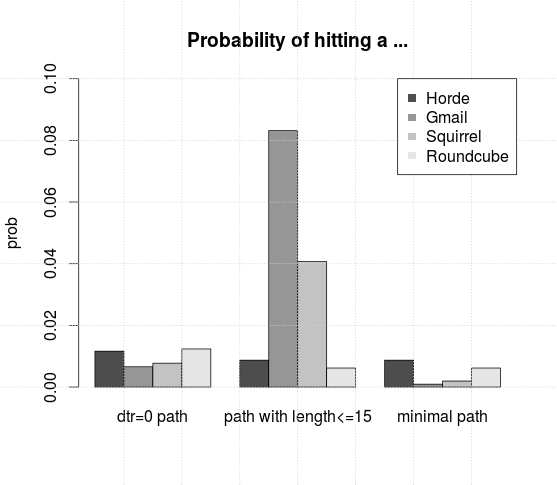
\includegraphics[width=\linewidth]{figures/prob-opt-path.png}
  \caption{Frequency of an optimal path.}
  \label{fig:freqopt}
\end{figure}

To combining these two results, we can easily compute the frequency of
paths with different length. Figure~\ref{fig:freqopt} shows, for each
application, the frequency of order 0 paths, the frequency of paths
with length less or equal to 15 (the minimum length across the four
applications), and the frequency of optimal paths (the shortest
ones). These values show that Gmail users have the lowest probability
to hit an order 0 path (because of the relative large number of order
1 paths made available by Gmail), have the highest probability to hit
a path with length 15 or less, have the lowest probability of hitting
the shortest paths.  Thus, flexibility and efficiency that can be
exploited with Gmail is counterbalanced by the required knowledge and
capability of chosing an optimal path. In other words, Gmail offers
many detours of order 1 which increase flexibility for some users and
might decrease effectiveness for other ones.


% >   d=0.050 # 20% chances that a user makes a generic mistake
% >   dprh=detour.page.rank(sc.hom,3,d);dprh
%          0          1          2          3 
% 0.73455373 0.11735984 0.05684419 0.09124223 
% >   dprg=detour.page.rank(sc.gom,3,d);dprg
%          0          1          2          3 
% 0.69210344 0.17697177 0.06228221 0.06864257 
% >   dprs=detour.page.rank(sc.sqm,3,d);dprs
%          0          1          2          3 
% 0.79062415 0.07122957 0.05364190 0.08450438 
% >   dprr=detour.page.rank(sc.rcm,3,d);dprr
%          0          1          2          3 
% 0.76538478 0.08355996 0.06247253 0.08858273 %

Another probabilistic analysis can be performed using page rank, which
can be used to compute the probability that a random walk in a graph
visits a certain vertex. We computed the page rank (with a damping
value of 5\% - meaning that the randowm walker with probability 5\%
jumps to an arbitrary state and probability 95\% chooses one of the
actions available in the current state) for each vertex in the graph,
and then added the page rank value for vertices with different detour order.
Figure~\ref{fig:pr} shows the resulting probabilities.


\begin{figure}
  \centering
  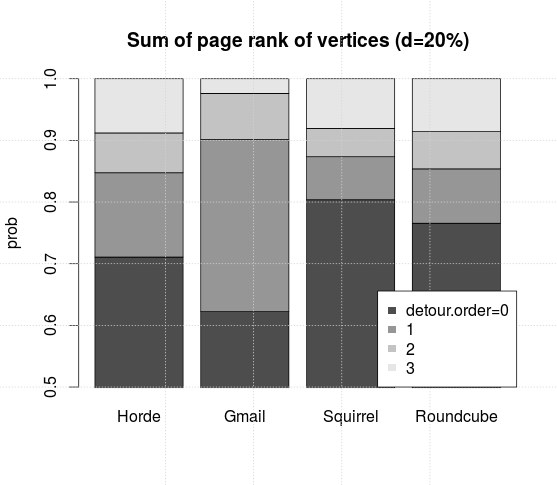
\includegraphics[width=\linewidth]{figures/pr.png}
  \caption{Probability that a random walk visits detour 0, 1, 2 or 3 states.}
  \label{fig:pr}
\end{figure}

With Gmail the probability of visiting an order 0 state is close to
70\%, the lowest among the four applications. But when it comes to
visiting an order 0 or 1 state, the probability increases to 87\%,
which is the highest. Thus, to compare Gmail with SquirrelMail, a
completely random usage of SquirrelMail has 10\% more probability of
hitting an error-free state than Gmail. That advantage is reduced when
considering order 0 and 1 paths, because with SquirrelMail the
probability is 85\% and Gmail it is 87\%.

Manual inspection of the shortest paths indicates that one reason of
the higher potential efficiency offered by Gmail is due to the
fact that users can start composing a new message while reading a
conversation, whereas in other applications an explicit ``closing'' of
the reading activity has to be performed. Another reason is in the
more streamlined process to attach a file: in Gmail one needs to
select the file(s) and they are automatically uploaded, whereas in
other applications one has to explicitly perform the uploading step
after selecting them.


\begin{figure}
  \centering
  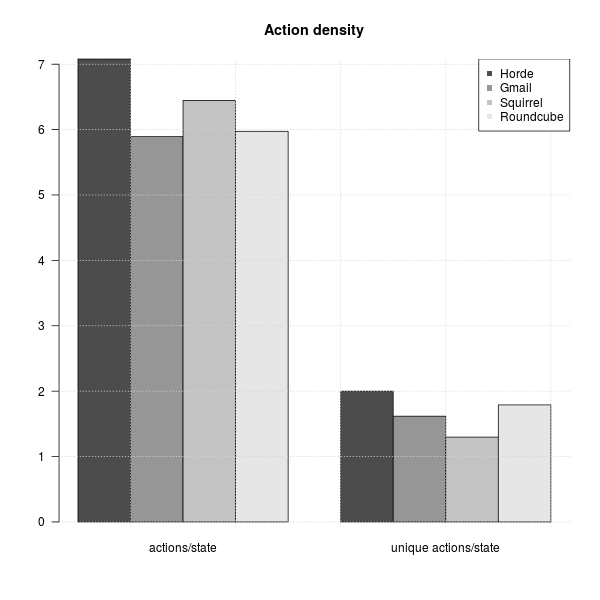
\includegraphics[width=\linewidth]{figures/ad.png}
  \caption{Action density.}
  \label{fig:ad}
\end{figure}

Figure~\ref{fig:ad} shows the \emph{action density} of the four
applications, in terms of average number of actions per state involved
in traces, and average number of \emph{unique} actions per state. The
former is an overall measure of the number of options that are made
available by a UI, the latter can be used to analyse how many
\emph{new} options the user is presented with in any state. For our
examples, the values are all in the range between 5.9 actions/state in
the case of Gmail and 7.1 for Horde, and 1.3 unique actions for
SquirrelMail and 2 for Horde. This suggests that Gmail features a more
compact design (fewer actions to do the same things), and SquirrelMail
is even more compact when it comes to the different types of actions;
thus it could be easier to learn.


\subsection{Comparing scenarios}

The same kind of analysis can be carried out to assess how suitable a
design is for a set of different scenarios. For example, a designer
might be interested in understanding what are some quantitative
differences in replying to a message as opposed to composing a new
one. 

For Horde, it turns out that composing a new message entails many more
order 0 paths (154 vs 86), and a comparable number of higher order
paths. The path length in the best case is the same across the two
scenarios, but in the average case composing has a length of 7.75
steps compared to 8.5 for reply. Probability of hitting an optimal
path is 4 times higher for compose.


This means that users will have a twice as much large choice of
correct paths when composing a new message rather than ``simply''
replying to a read one. On average, when composing, users could be
9\% more efficient, and they are 4 times more likely to do the right
things. Thus, Horde is more suitable for composing new messages than
it is for replying to existing ones.

\subsection{Adding features}

Execution traces can be used also to assess what is the effect of
adding a widget or feature to an existing UI.  For example, we studied
the cruise control features of cars. One of the examples is system S,
where the driver can engage the system, and once it is engaged, speed
can be increased or decreased with small or large steps. Of course the
system can also be disengaged (by pressing the brake pedal, for
example).
System A is more elaborate, as it includes also a memory function:
when it is disengaged it remembers the current speed, which can be
recalled later on.  There are two ways to re-engage it: one
by setting a new speed, and one by recalling the previous one. In
addition,  if the car drives for more than 5 minutes at a higher
speed than the set one, system A automatically disengages.

Thus, one possible design question is ``What are the effects of adding
these functionalities?'' in a typical driving scenario where a speed
is selected, then the system is disengaged, and then the same speed
needs to be set? 

System S (where we assumed that re-setting the speed is done manually
by the driver with 4 actions on ``up'' and ``down'' to get
approximately get the same speed) leads to 1 order 0 path requiring 7
steps; there are 8 order 1 paths with average length  9.4. The
probability of hitting the optimal path is 0.11; action density is
1.75, and unique action density is 1.25.

On the other hand, system A has 2 order 0 paths (average length 4.5),
and 7 order 1 paths (average length 6.8). 
The optimal path probability is 0.06; action density is
2.2, and unique action density is 1.2.

In both cases the reasons for detours deal with the possibility of
disengaging the system at the wrong moment.

Therefore we can conclude that:
\begin{inparaenum}
\item system A makes users more efficient;
\item with A there are two possible ways to achieve the scenario, thus
  more flexibility is given;
\item with A the probability of doing the right thing is almost half
  of system S: it might be more difficult to do the right thing
  because more possibilities are offered;
\item system A features a more compact design, with fewer action types
  to be performed at each moment, being therefore potentially easier
  to learn and remember.
\end{inparaenum}


\hl{present them in terms of :
consistency,
error proneness, efficiency, premature committment, flexibility}


\clearpage





% \begin{table*}[ht]
% \centering
% \begin{tabular}{rllll}
%   Step &Horde & Gmail & Squirrel & Roundcube\\
%   \hline
%   1 & openMessage(msg) & open(conversation) & openMessage(msg) & openMessage(msg) \\ 
%   2 & exitMessage & goBack & exitMessage &  exitMessage \\ 
%   3 & openMessage(msg) & open(conversation) & openMessage(msg) & openMessage(msg) \\ 
%   4 & reply & reply & reply & reply \\ 
%   5 &  typeBody & typeBody & typeBody                       &  typeBody \\ 
%   6 &  send &  send & send                                  & send \\ 
%   7 &  exitMessage &  & exitMessage                  &  exitMessage \\ 
%   8 & compose &compose & compose                        & compose \\ 
%   9 & addReceiver(receiver) &  addReceiver(receiver)  & addReceiver(receiver)   & addReceiver(receiver) \\ 
%   10 & browseFiles          & attachFiles   & browseFiles  & attachAFile \\ 
%   11 & selectAttachments(file) & open(files)  & selectAttachments(file)          &  selectAttachments(files) \\ 
%   12 & update                &  &add   &  upload \\ 
%   13 &  typeSubject          &  typeSubject          &  typeSubject & typeSubject \\ 
%   14 & typeBody &         typeBody                    & typeBody     & typeBody \\ 
%   15 &  send &           send                    &  send        &  send \\ 
%    \hline
% \end{tabular}
% \end{table*}


\section{Discussion}
\label{sec:discussion}

\hl{dire} di SEPARATING concerns, ad es M-V-C, per vedere le
  implicazioni di ciascuna e non soffrire di ``saturation'', vedi adams

dire che le ns analisi sono prive di assunzioni su conoscenze
abilita'; le probability sono puramente sulla base delle frequenze.

dire di cogtools: noi non prevediamo i tempi (richiede modeling
psicologico e dei specifici widgets). pero' forniamo un'analisi che
puo' guidare chi applica cogtool.

dire di horrocks \cite{horrocks99}

dire di agile modeling \cite{ambler02}

issues dealing with complexity of searching paths

\section{Conclusion}
\label{sec:conclusion}





% REFERENCES FORMAT
% References must be the same font size as other body text.
\bibliographystyle{SIGCHI-Reference-Format}
\bibliography{gb,database}

\end{document}

%%% Local Variables:
%%% mode: latex
%%% TeX-master: t
%%% End:
